We crawled Twitter data using Twitter Streaming API for two years spanning 2013 and 2014 years. 
%This type of crawling provides us with a very sparse set of data, roughly $1\%$ of all tweets \footnote{\hyperref[]{http://allthingsd.com/20101110/twitter-firehose-too-intense-take-a-sip-from-the-garden-hose-or-sample-the-spritzer|}}. 
The total number of tweets collected is $829,026,458$. In the context of Twitter, we consider a list of $5$ features for each tweet. Each tweet has a $From$, the person who tweeted it, and a $Time$ which is the date information of the tweet. It can also contain 
\begin{itemize}
\item $Hashtag(s)$, keywords specified using \# sign
\item $Mention(s)$, another Twitter username being mentioned using @ sign
\item $Term(s)$, uni-grams which we extract from the 140 characters of the tweet. %These uni-grams are later cleaned to remove $Term$s with no meaning (total number of $Term$s before cleaning was $20,234,729$)
\end{itemize}
We provide more detailed statistics about each feature in Table ~\ref{table:featureStatistics} and Table ~\ref{table:featureUnique}. Here, we provide the unique number of the feature in our dataset, in addition to maximum, average, and median values of each feature across the tweets, user, and hashtag dimensions. For example, a hashtag has been used in average by $10.08$ users or users have used $2$ hashtags on average.

For $Location$ feature, Fig ~\ref{fig:choropleths} shows the distribution of tweets across different U.S. and international locations for $3$ chosen topics which we found to be more interesting due to their geographical distribution over various locations. For example, we can see that Middle east and Malaysia stand out for the topic of Human Caused Disaster. Malaysia is a hot place for this topic due to MH370 incident with lots of usage of \#whereisthefuckingplane.

%%%%%%%%%%%%%%%%%%%%%%%%%%%%%%%%%%%%%%%%%%%%%%%%%%%%%%%%%%%%%%%%%%%%%%%%%%%
\begin{figure*}[!tbh]
\centering
\begin{tabular}{ccc}
\begin{tabular}{ccc}
\subfloat[Fig:][Human Caused Disaster]{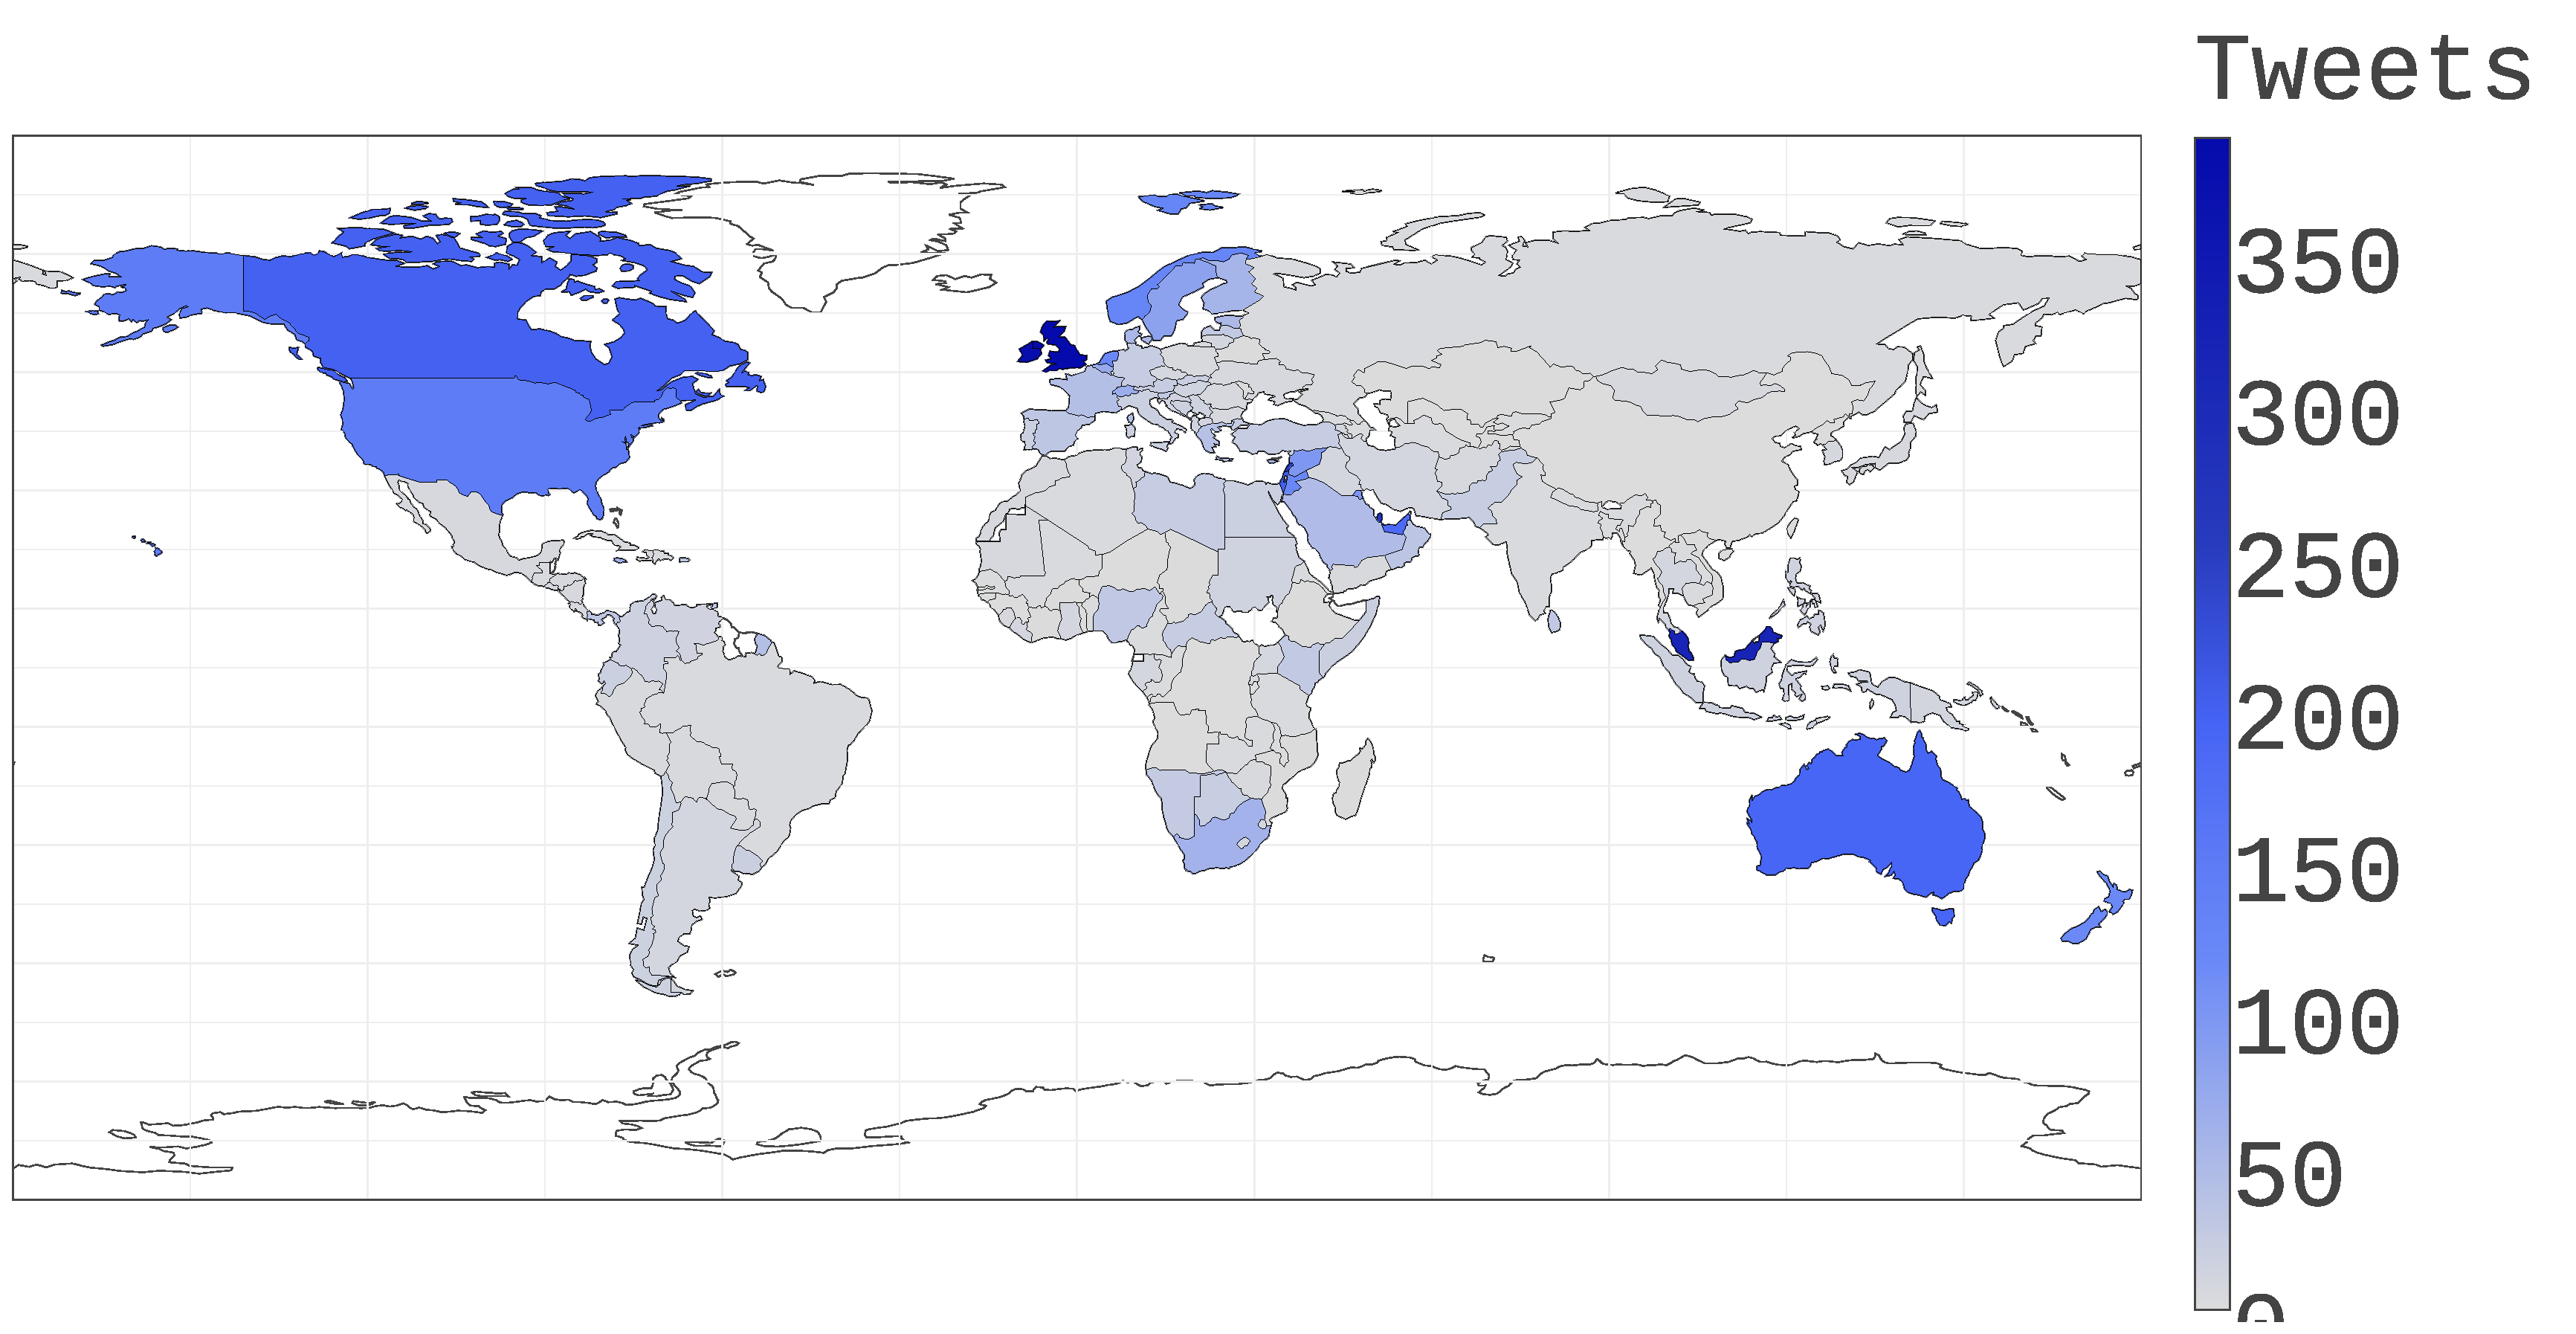
\includegraphics[width=5.3cm]{images/location/world/socialsensor-world-HumanCausedDisaster_location.eps}}
\subfloat[Fig:][Iran Deal]{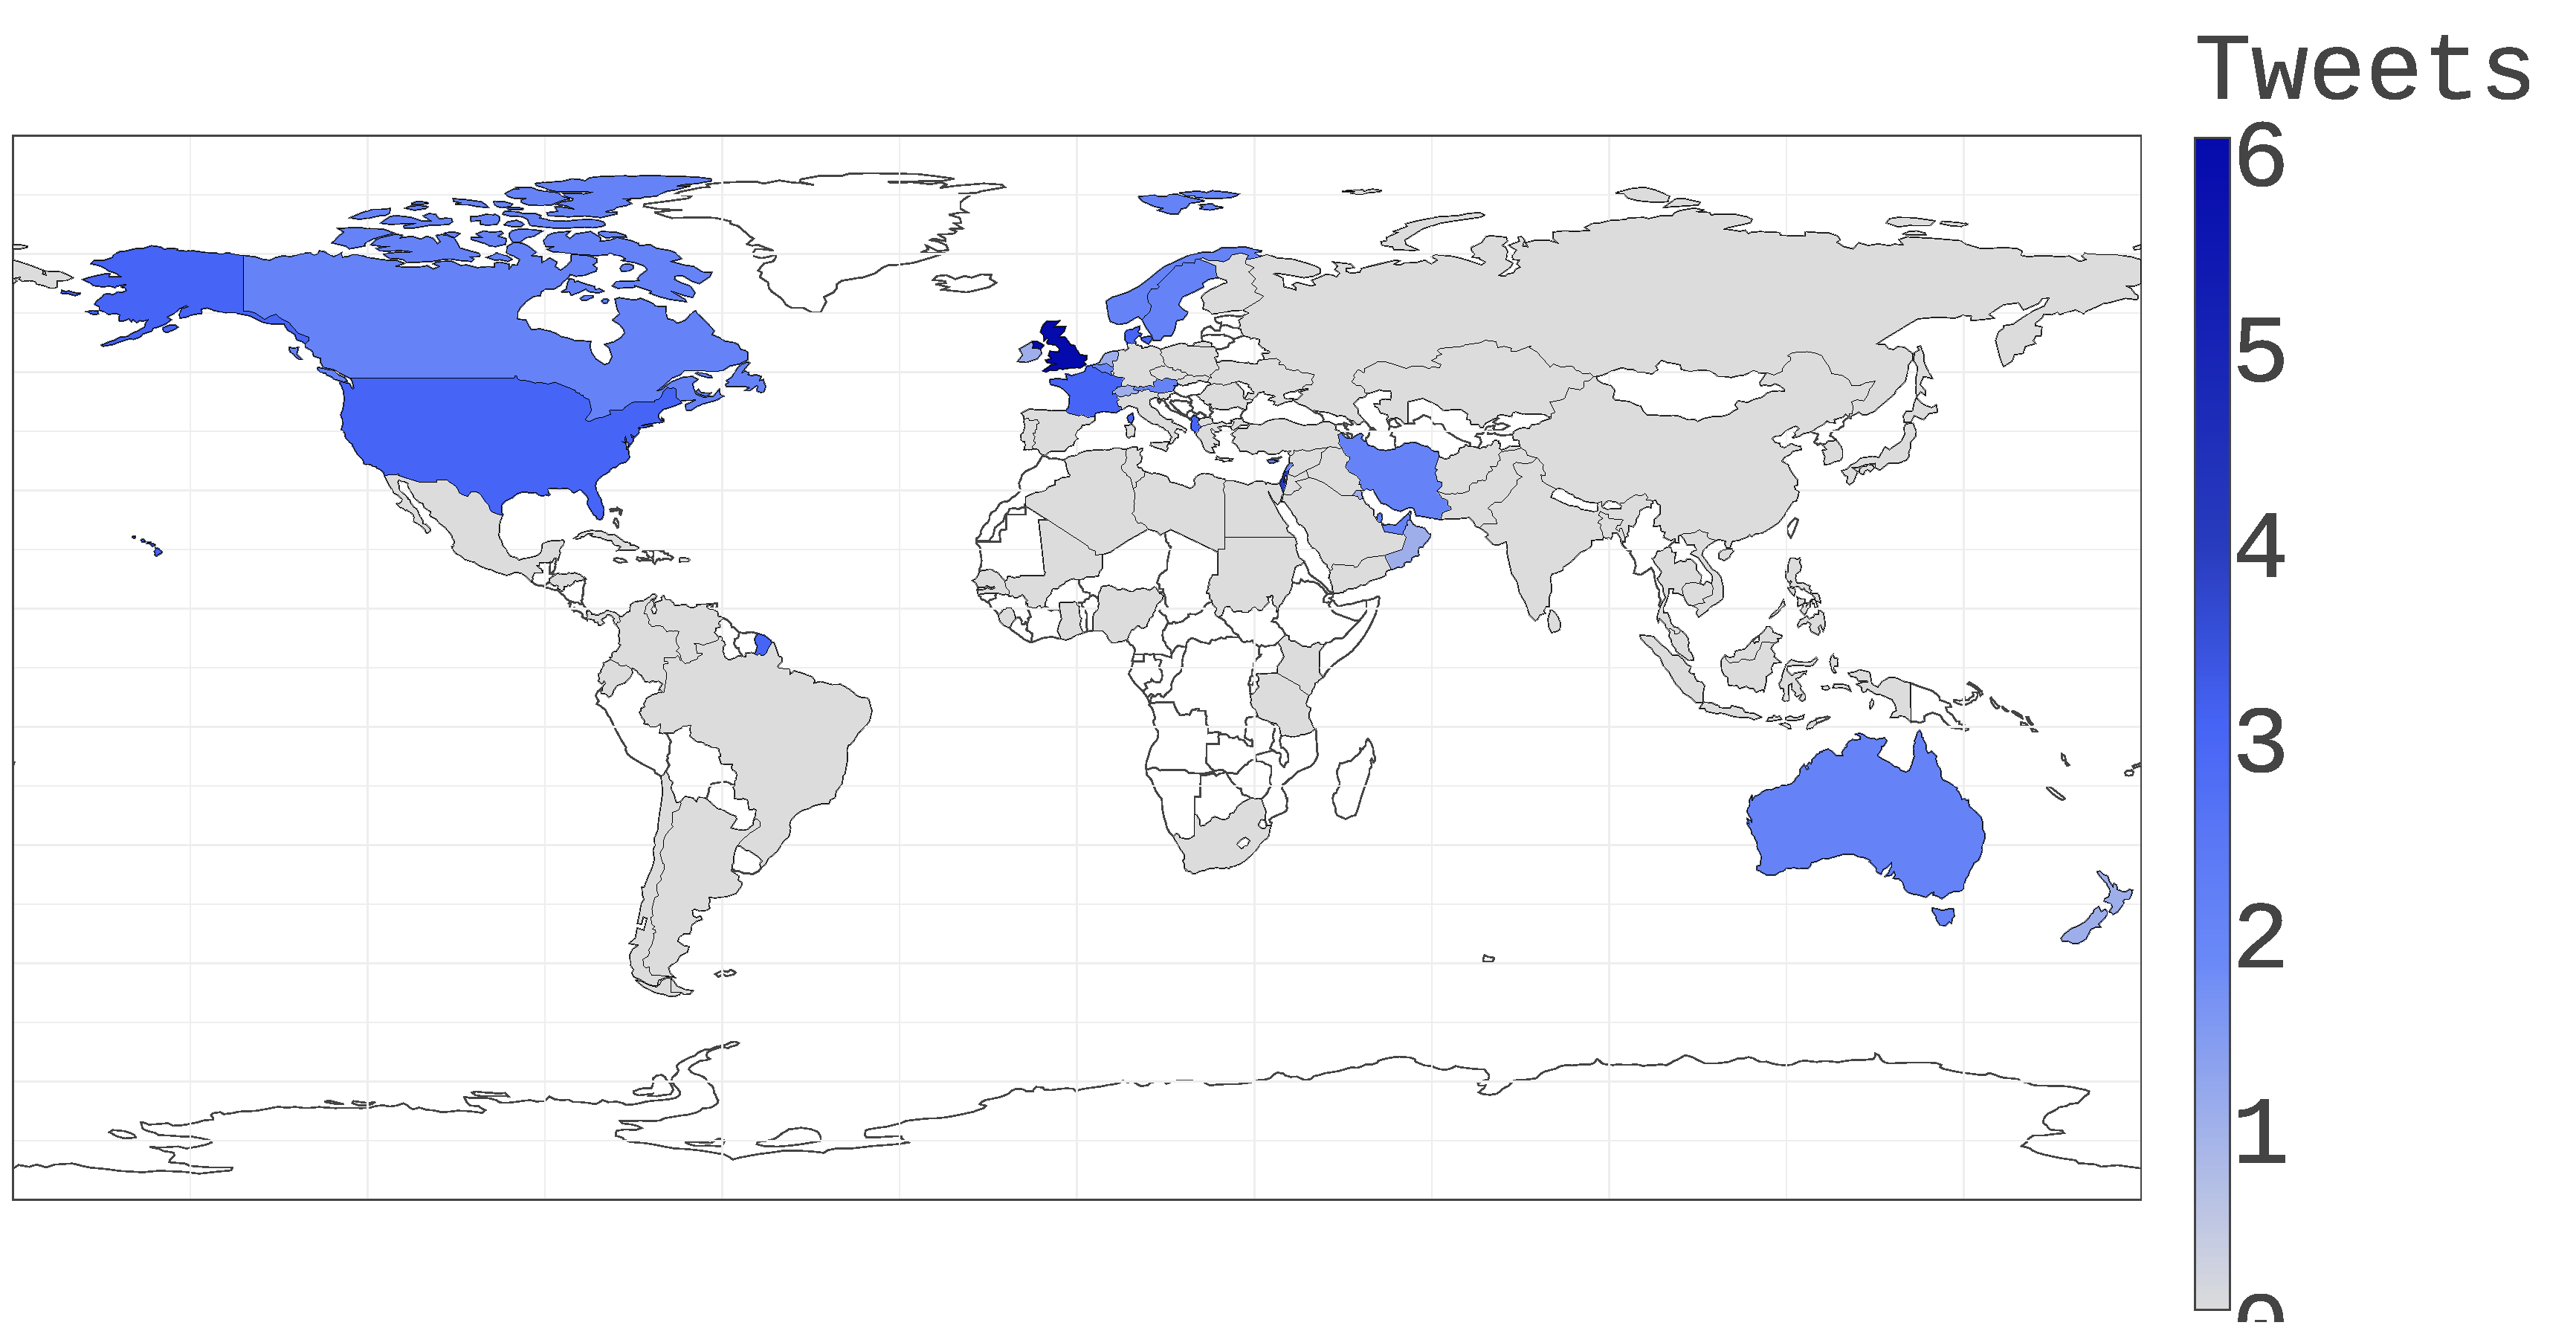
\includegraphics[width=5.3cm]{images/location/world/socialsensor-world-irannucleardeal_location.eps}}
\subfloat[Fig:][Soccer]{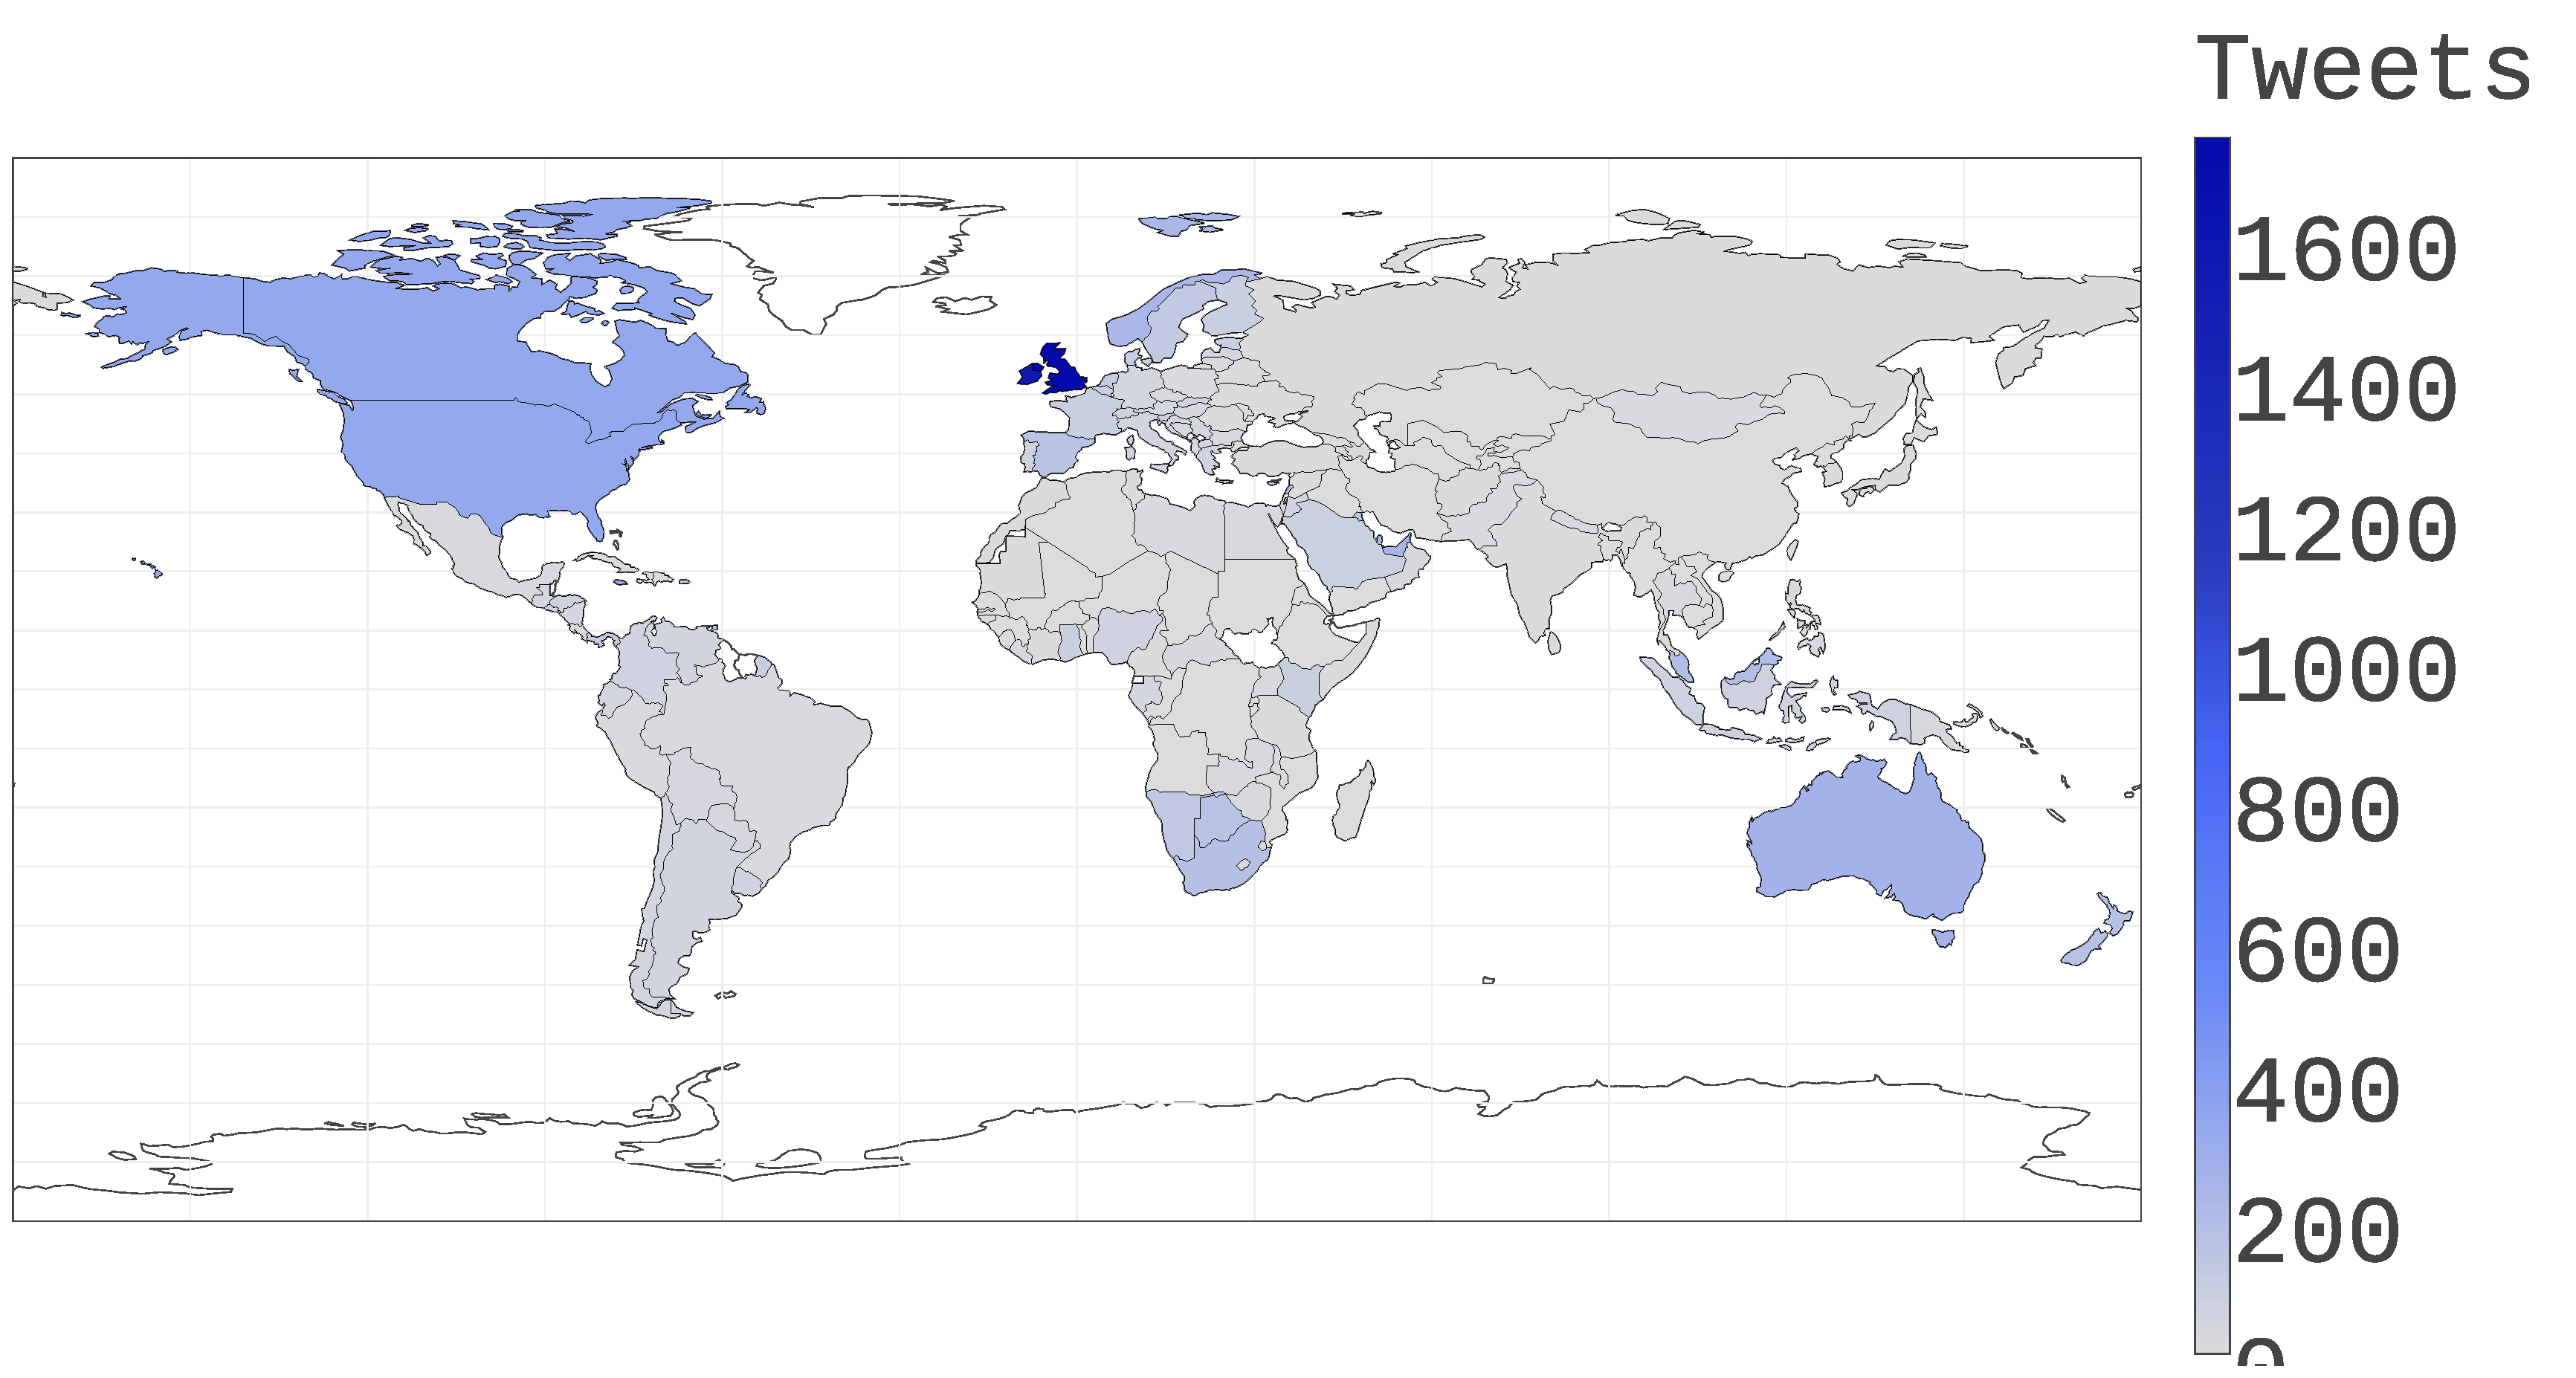
\includegraphics[width=5.3cm]{images/location/world/socialsensor-world-soccer_location.eps}} \\
%\vspace{-10mm}
\subfloat[Fig:][Health Epidemics]{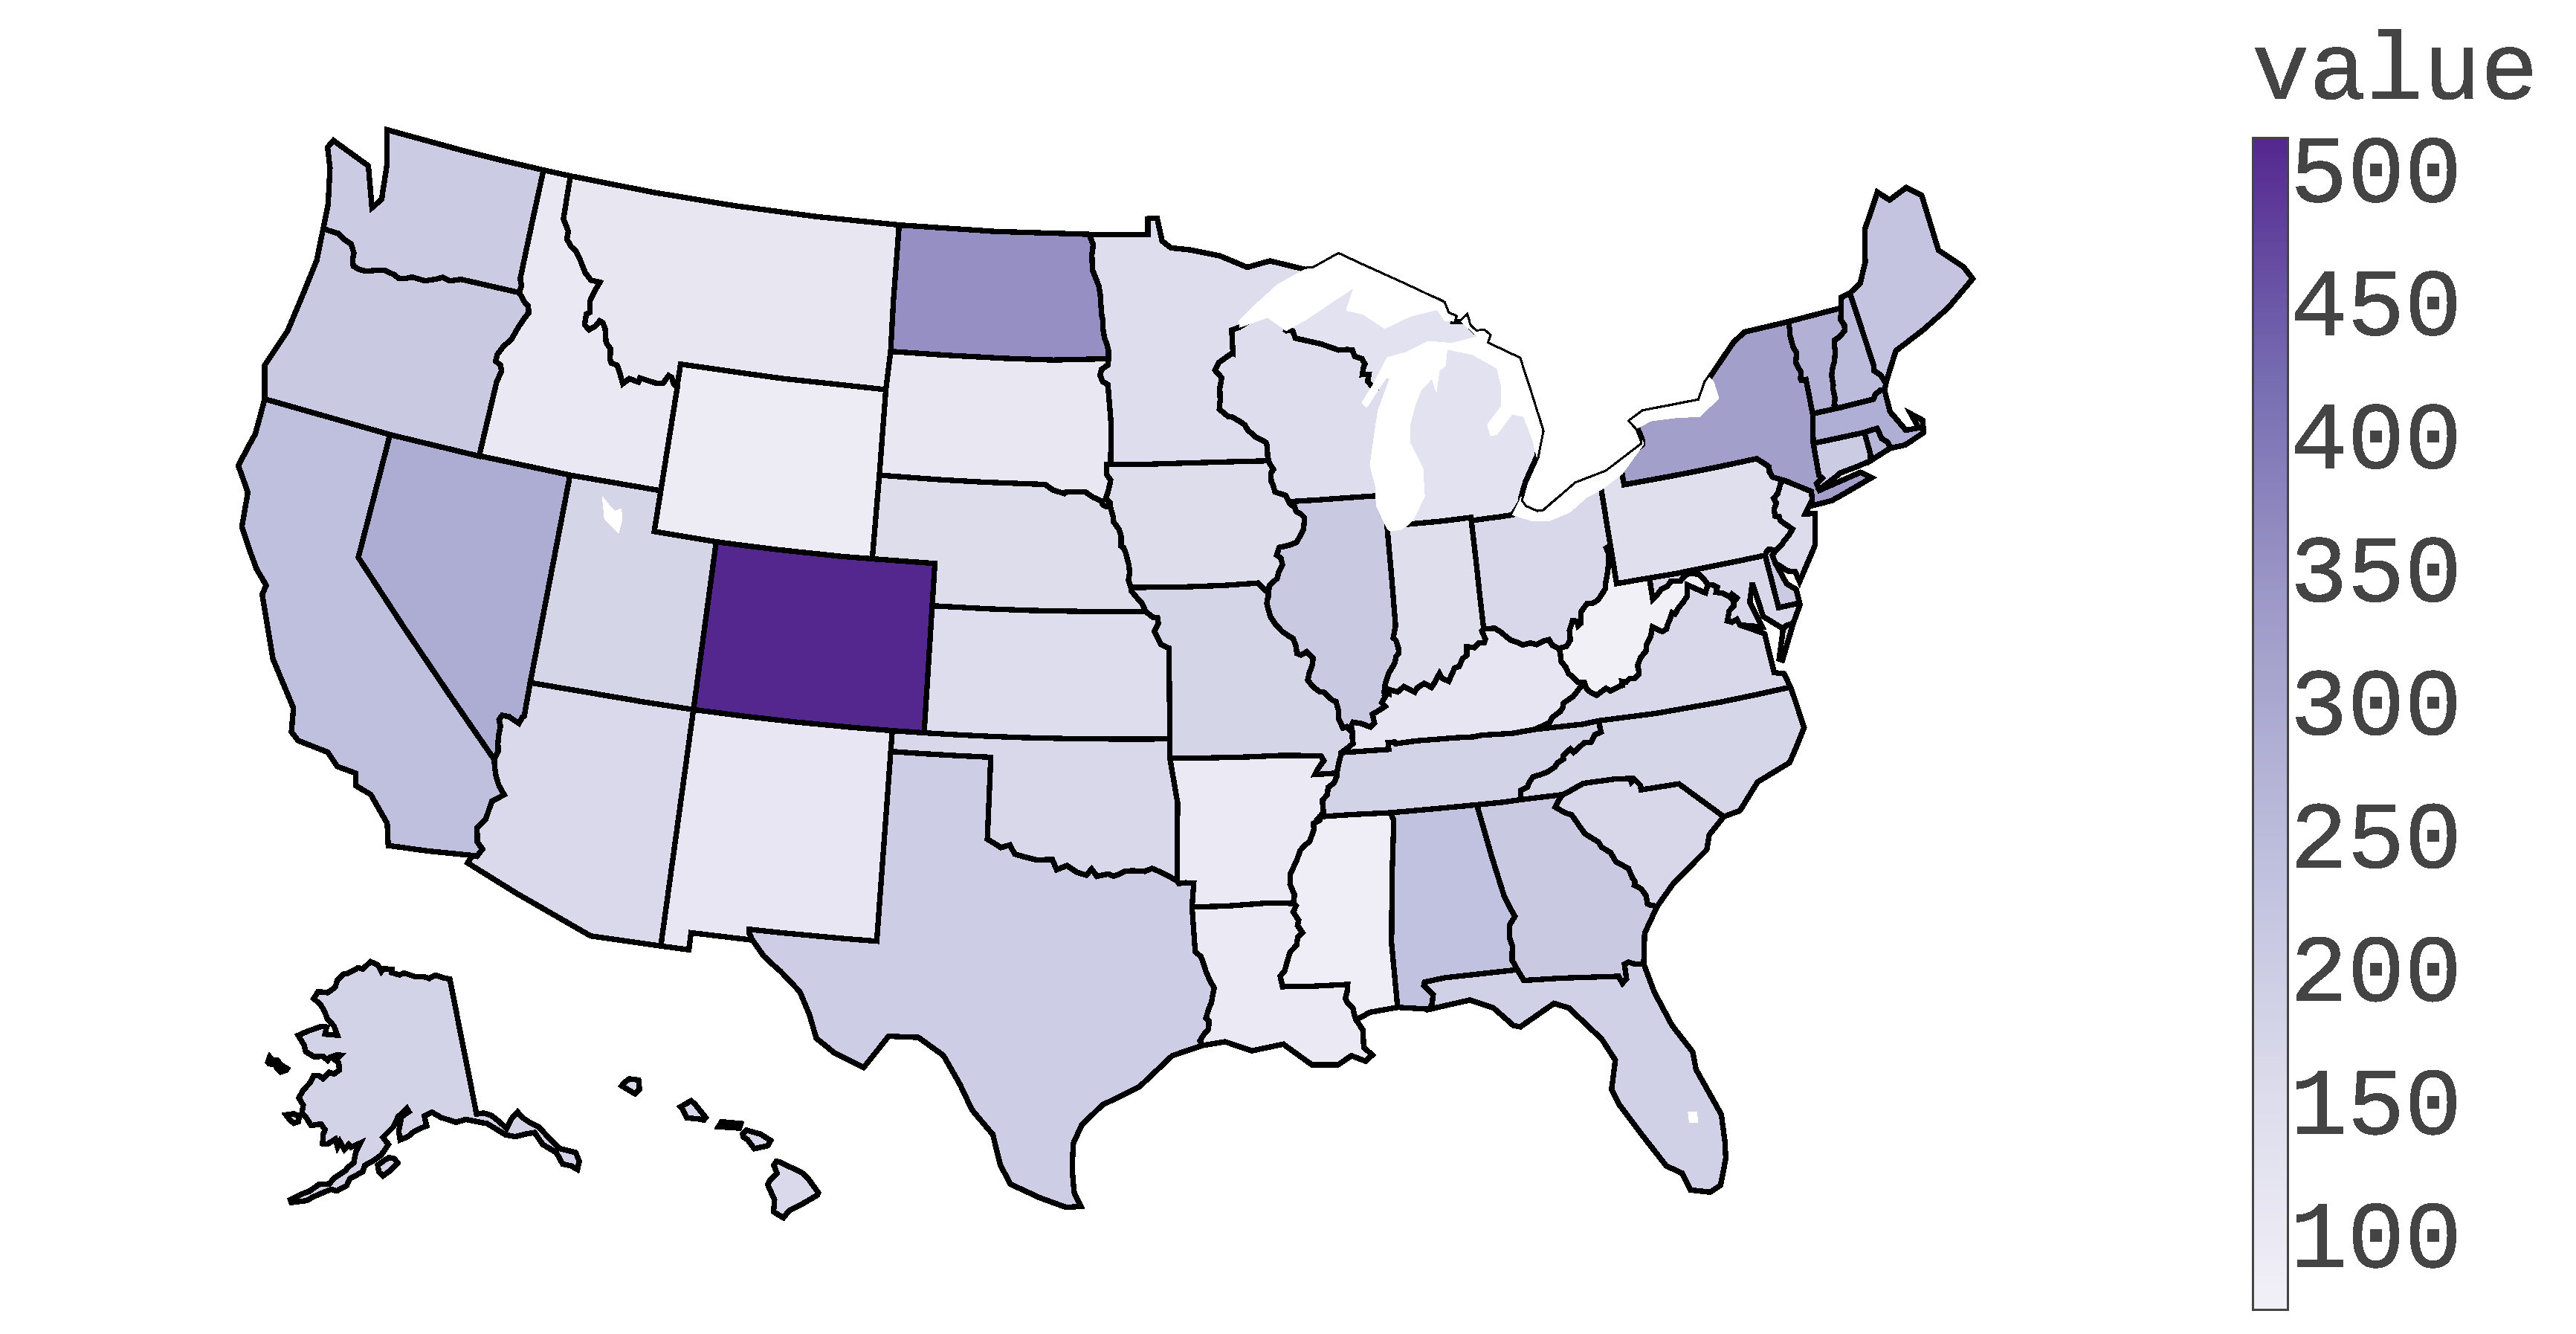
\includegraphics[width=5.3cm]{images/location/states/SocialSensor-us-states-health_epidemics_location.eps}}
\subfloat[Fig:][Social Issues]{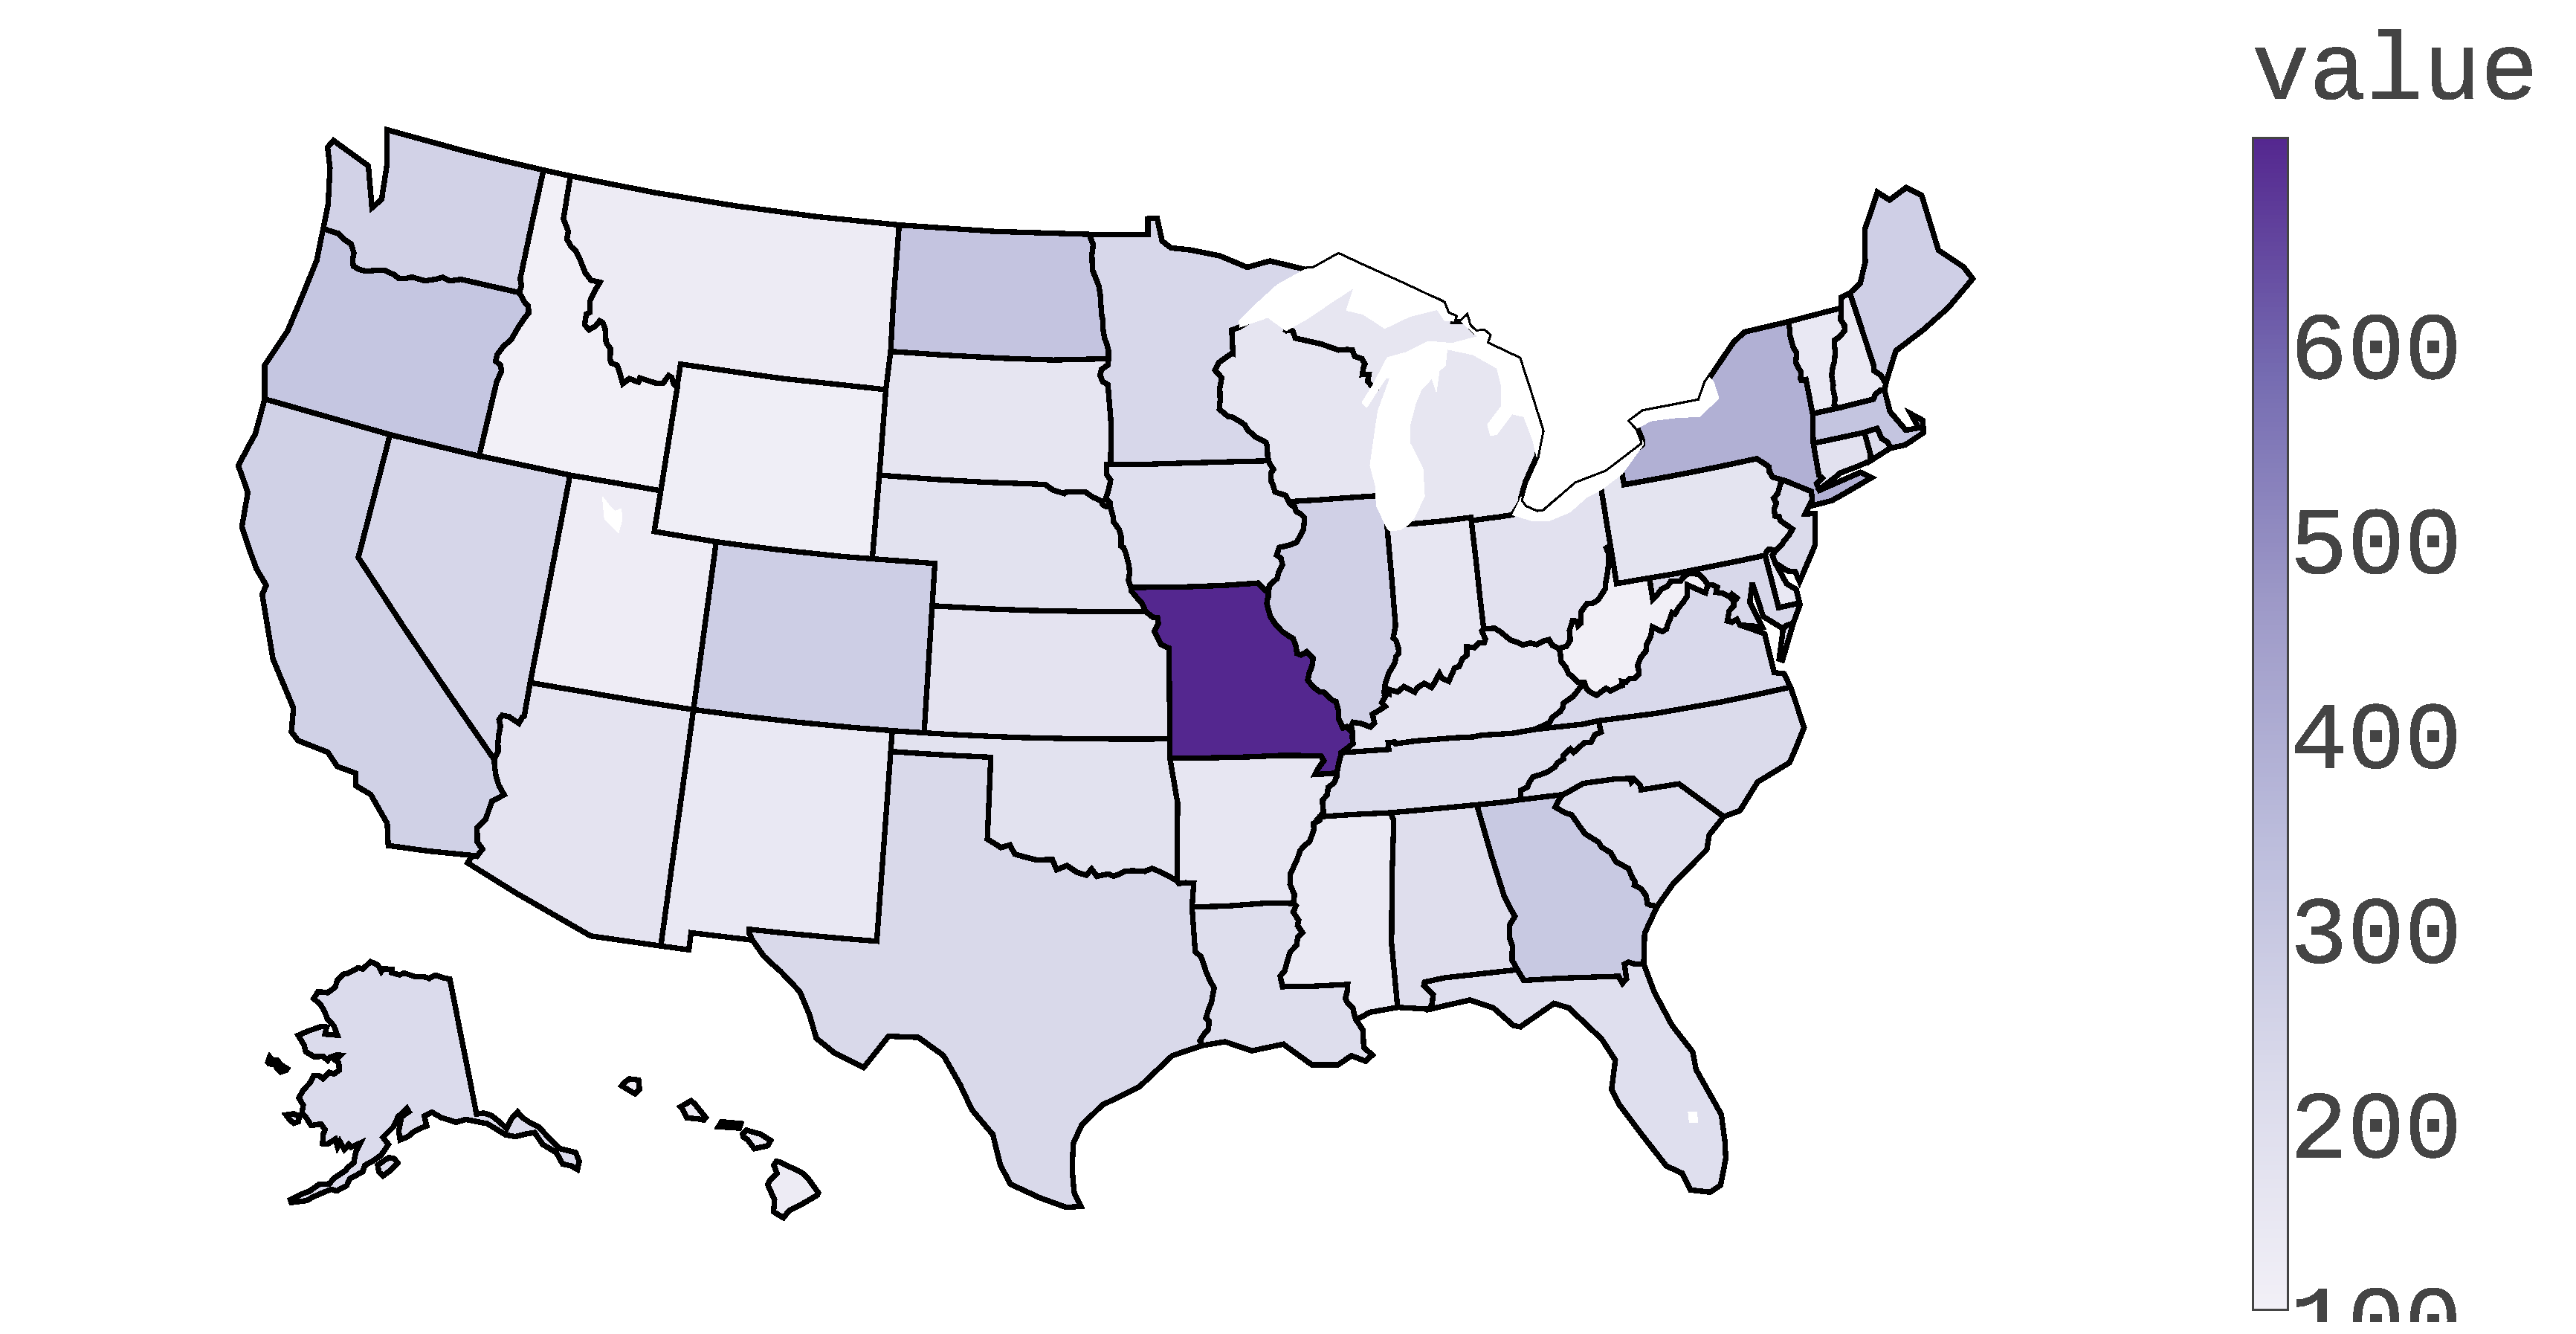
\includegraphics[width=5.3cm]{images/location/states/SocialSensor-us-states-socialissues_location.eps}}
\subfloat[Fig:][Space]{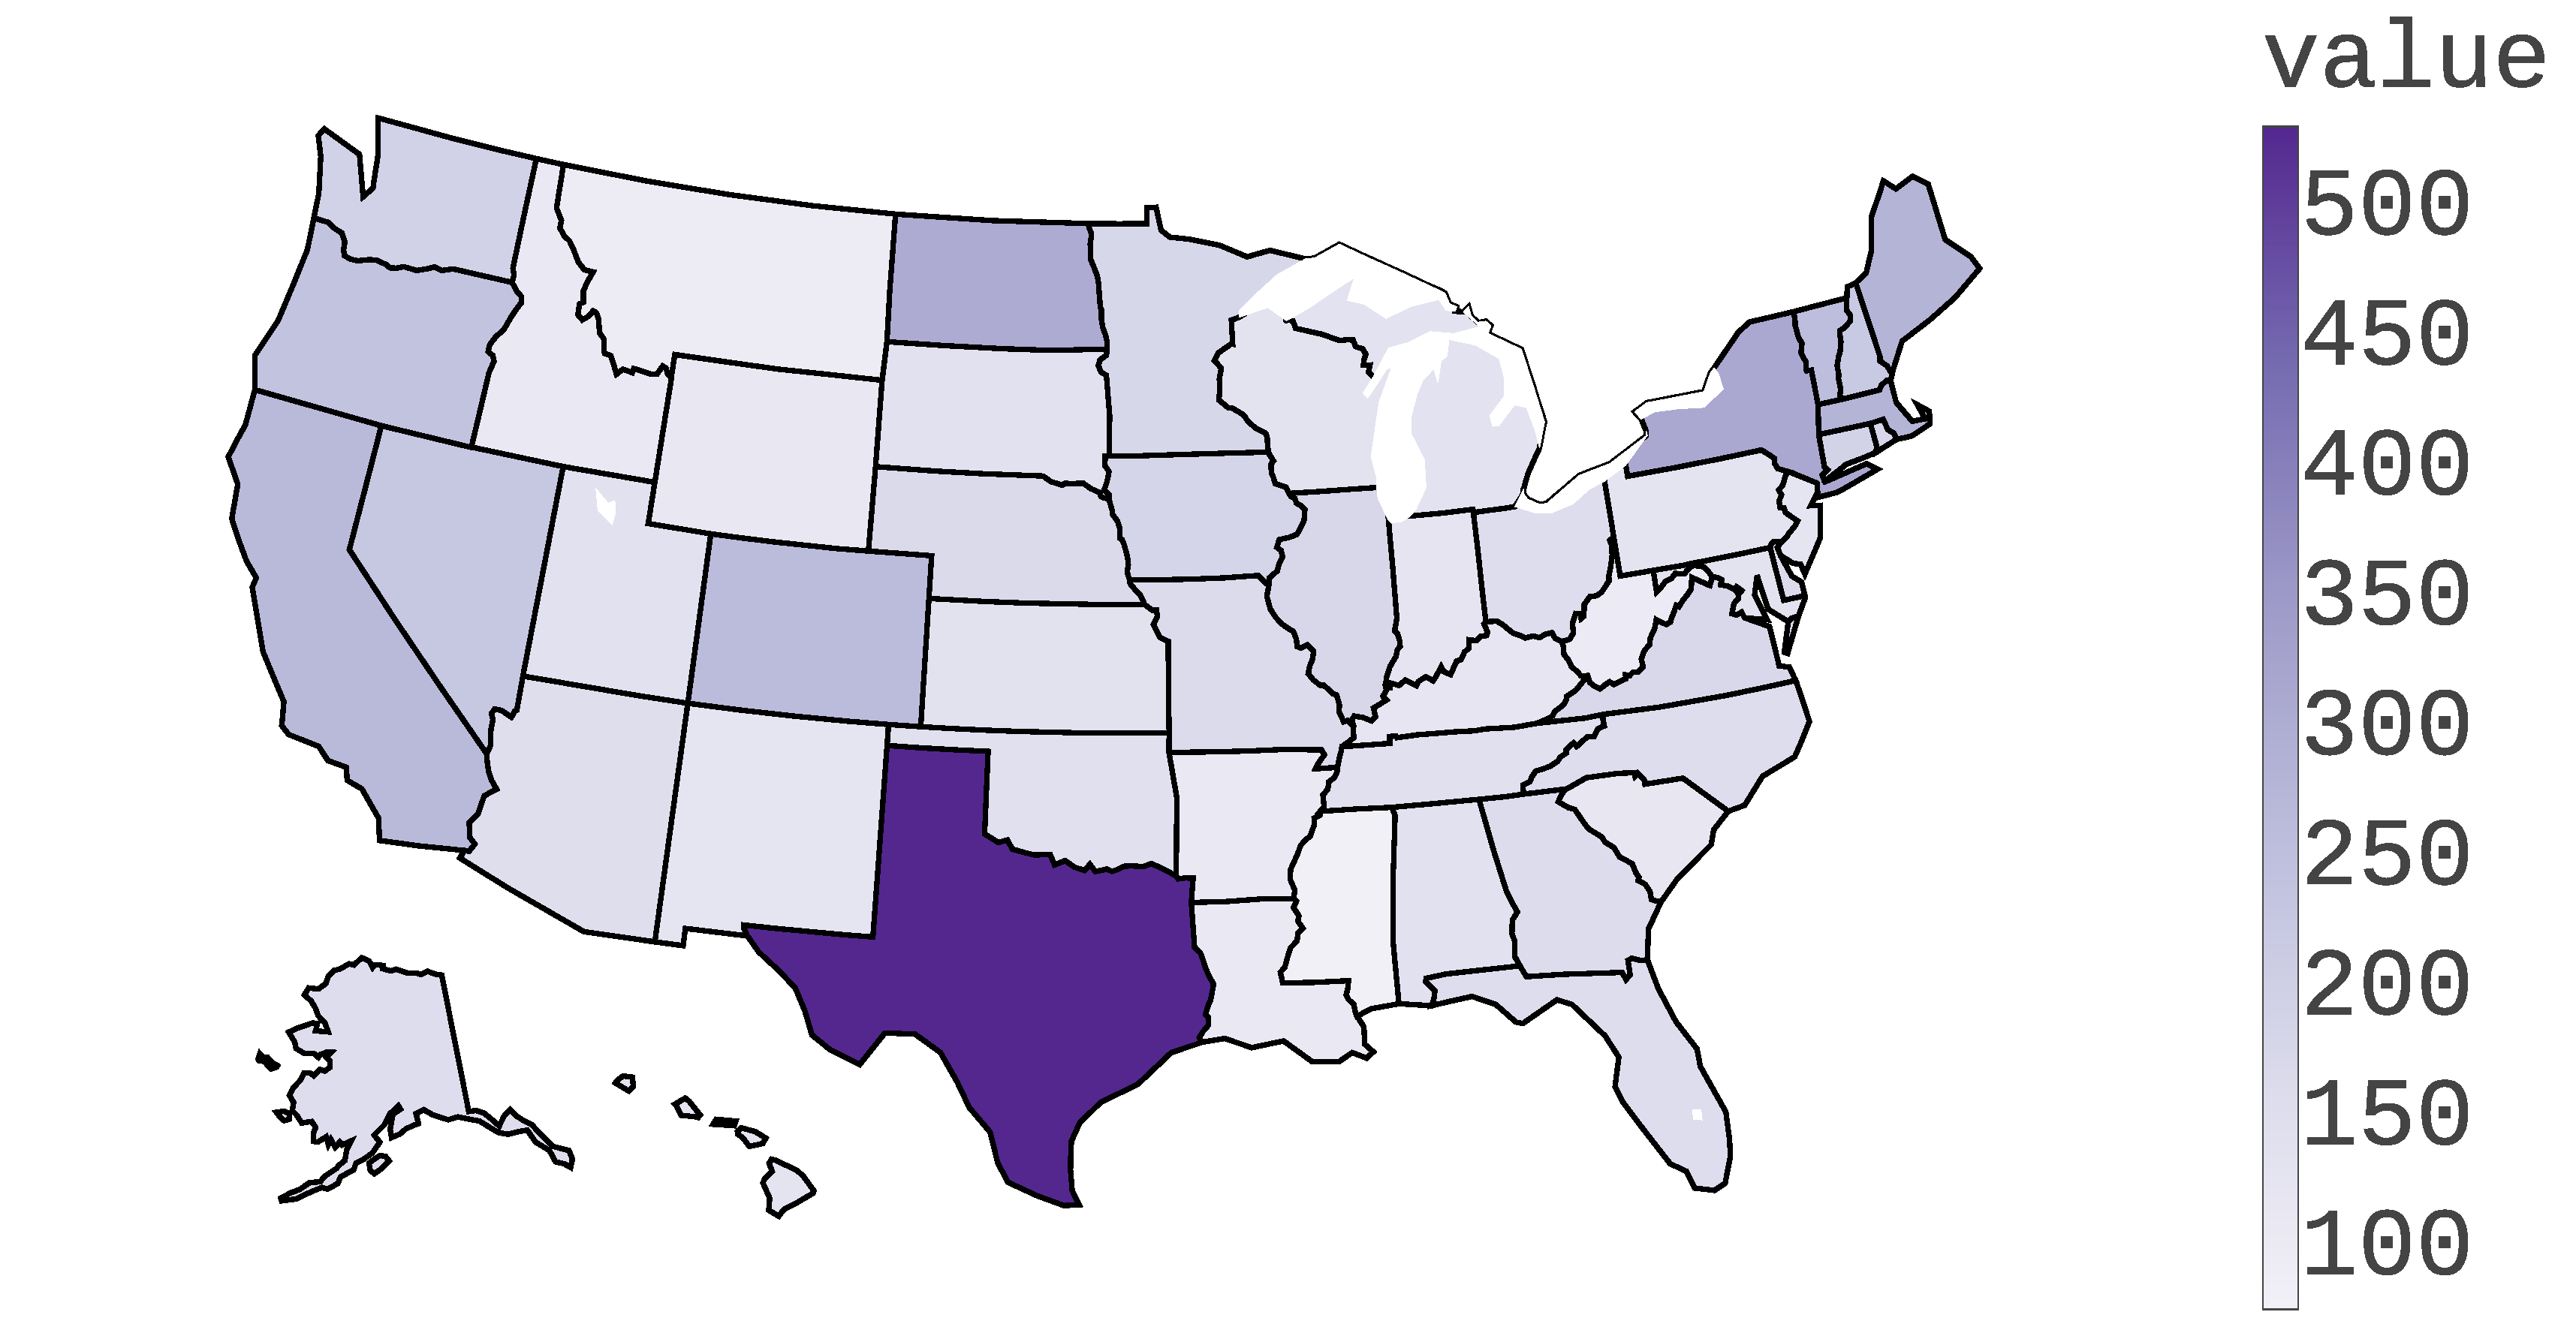
\includegraphics[width=5.3cm]{images/location/states/SocialSensor-us-states-space_location}} \\
\end{tabular}
\end{tabular}
\vspace{-2mm}
\caption {Distribution of tweets across International locations (top row) and U.S. locations (bottom row)}
\label{fig:choropleths}
\end{figure*}
%%%%%%%%%%%%%%%%%%%%%%%%%%%%%%%%%%%%%%%%%%%%%%%%%%%%%%%%%%%%%%%%%%%%%%%%%%%

%%%%%%%%%%%%%%%%%%%%%%%%%%%%%%%%%%%%%%%%%%%%%%%%%%%%%%%%%%%%%%%%%%
\begin{table}[th!]
\centering
{\renewcommand{\arraystretch}{1.2}
\resizebox{0.5\textwidth}{!}{%
\begin{tabular}{|l|c|c|c|c|}
\hline
\multicolumn{5}{|c|}{\textbf{Used in \#Tweets}} \\ \hline
\textbf{Feature} & \textbf{Max} & \textbf{Avg} & \textbf{Median} & \textbf{Max entity} \\ \hline
\textbf{From} & 10,196 & 8.67 & 2 & running\_status \\ \hline
\textbf{Hashtag} & 1,653,159 & 13.91 & 1 & \#retweet \\ \hline
\textbf{Mention} &  &  &  &  \\ \hline
\textbf{Location} &  &  &  &  \\ \hline
\textbf{Term} & 241,896,559 & 492.37 & 1 & rt \\ \hline \hline
\multicolumn{5}{|c|}{\textbf{Used by \#Users}} \\ \hline
\textbf{Hashtag} & 592,363 & 10.08 & 1 & \#retweet \\ \hline
\textbf{Mention} & 26,293 & 5.44 & 1 & dimensionist \\ \hline
\textbf{Location} & 739,120 & 641.5 & 2 & london \\ \hline
\textbf{Term} & 1,799,385 & - & 1 & rt \\ \hline \hline
\multicolumn{5}{|c|}{\textbf{Using \#Hashtags}} \\ \hline
\textbf{From} & 18,167 & 2 & 0 & daily\_astrodata \\ \hline
\end{tabular}
}}
\caption{Feature Statistics of $829,026,458$ tweets in our Twitter dataset}
\label{table:featureStatistics}
\end{table}

\begin{table}[th!]
\centering
{\renewcommand{\arraystretch}{1.2}
\resizebox{0.5\textwidth}{!}{%
\begin{tabular}{|l|c|c|c|c|c|}
\hline
 & \textbf{From} & \textbf{Hashtag} & \textbf{Mention} & \textbf{Location} & \textbf{Term} \\ \hline
\textbf{\#Unique} & 95,547,198 & 11,183,410 & 411,341,569 & 58,601 & 20,234,728 \\ \hline
\end{tabular}
}}
\caption{Number of unique values for each feature of $829,026,458$ tweets in our Twitter dataset}
\label{table:featureUnique}
\end{table}
%%%%%%%%%%%%%%%%%%%%%%%%%%%%%%%%%%%%%%%%%%%%%%%%%%%%%%%%%%%%%%%%%%